
\chapter{实验结果与分析}
\label{chap:result}

\section{算法实现}
\label{sec:implementation}

我们使用了Python编程语言对算法进行了实现。下面介绍一些实现中值得注意的部分。

\subsection*{参数的设置}
\label{sec:config}

模拟退火算法对参数设置是非常敏感的,包括初始温度的设置,降温的速度,评价函数的设计都会对最后收敛的速度和结果有比较大的影响。经过反复试验,我们确定了以下的参数设置:

\begin{itemize}
\item \textbf{初始温度}。由于在判断是否接受时计算了$\Delta value/t$的值,因此我们希望能将温度和评价归一化。初始温度被设置为初始评价的$K$倍,$K = N_v N_p$。
\item \textbf{降温速度}。降温速度太快会导致算法很快收敛,得不到比较理想的结果,而降温速度太慢则会导致收敛过程很长,并且在计算初期接受过于不理想的结果,影响效率。经过试验,使用了$t_{n+1} = 0.89t_n$这样的线形降温速度,收到了良好的效果。
\item \textbf{评价函数}。在实现中采用了四种因素综合评价的方式。我们考虑了PM的数量,RAM的负载均衡,CPU的负载均衡和平均冲突率,并以这四个值的乘积作为评价函数的返回值。\label{evalutation}
\end{itemize}

\subsection*{评价函数}
\label{sec:evaluation-function}

在所有参数中,评价函数的确定是对算法影响最大的,因为它直接决定了算法的走向。比如我们选取使用PM的数量作为评价的标准,那么在迭代的过程中接受那些使用更少PM的解。如前文所说,我们希望综合考虑更重因素,所以我们采用了如下的评价函数:

\begin{itemize}
\item \textbf{PM的数量}。我们用\texttt{count\_active(plist)}函数来评价。函数接受一个根据状态生成的PM信息列表,计算其中被``激活''(有VM部署在其上)的PM的个数(为了不同规模数据间的比较,实际返回的是PM的个数与$N_v$的比例。
\item \textbf{RAM的均衡负载}。我们用\texttt{ram\_stdev(plist)}函数来评价。函数接受一个根据状态生成的PM信息列表,计算RAM利用率的均方差(Standard Deviation)。如果RAM利用率的均方差的足够小则说明每台PM上的RAM负载比较均衡。
\item \textbf{CPU的均衡负载}。和RAM的均衡负载类似,我们用\texttt{cpu\_stdev(plist)}函数来评价。函数接受一个根据状态生成的PM信息列表,计算CPU利用率的均方差。如果RAM利用率的均方差的足够小则说明每台PM上的CPU负载比较均衡。
\item \textbf{平均冲突率}。我们定义平均冲突率$\mu \geq 1$,使用\texttt{count\_conficts(plist)}函数来计算。函数接受一个根据状态生成的PM信息列表,结算其中RAM利用率超过$1$的PM的平均RAM利用率。如果不存在利用率超过$1$的PM,则取值$1$.
\end{itemize}

\subsection*{测试数据的选取}
\label{sec:data}
通常,云计算服务提供商提供的用户的选择都是有限的,比如提供给用户选择``双核500MB内存'',通过限制虚拟机请求的数据可以针对性的优化部属算法。在这种情境下,\texttt{First-Fit}算法通常能收到良好的效果。

在本文所描述的情境中,为了更好的模拟不同情境下算法的效果,我们没有对请求的数据进行限制(但是为了避免无解的情况,对数据的上下限进行了规定)。我们尝试了多种测试数据生成的方法,最终确定以下的测试数据:
\begin{itemize}
\item 每组测试设计都是\textbf{随机}生成的。
\item 将$C^T$设置为$8$,即认为每个实体机都具有$8$个计算核心;将$R_T$设为$1$。
\item $C^{req}_i$将取$0.1-8.0$之间的随机数;$R^{req}_i$取$0.2-0.8$之间的随机数;$E_i$取$0.2-0.8$之间的随机数。生成的数据可以认为即包含运算需求高的请求也包含存储需求高的请求。
\item 测试数据的数量取$100-1000$间隔$100$的整数,用以模拟不同规模下的请求。
\end{itemize}

在随机的数据和不同的数据规模上的得到相似测试结果可以从某种程度上证明算法的稳定性和可行性。通过不同数据规模和多次试验,我们得出了相应的结论,并且与\texttt{First-Fit}算法在同样的数据上的结果进行了比对。

\section{有效性}
图\ref{fig:feas}是算法在$N_v = 200,N_p = 200$时的迭代情况,我们看到算法最终收敛在一个比较好的解上。在所有测试中算法均能成功收敛在一个解上。
\begin{figure}[htbp]
\centering %图形居中
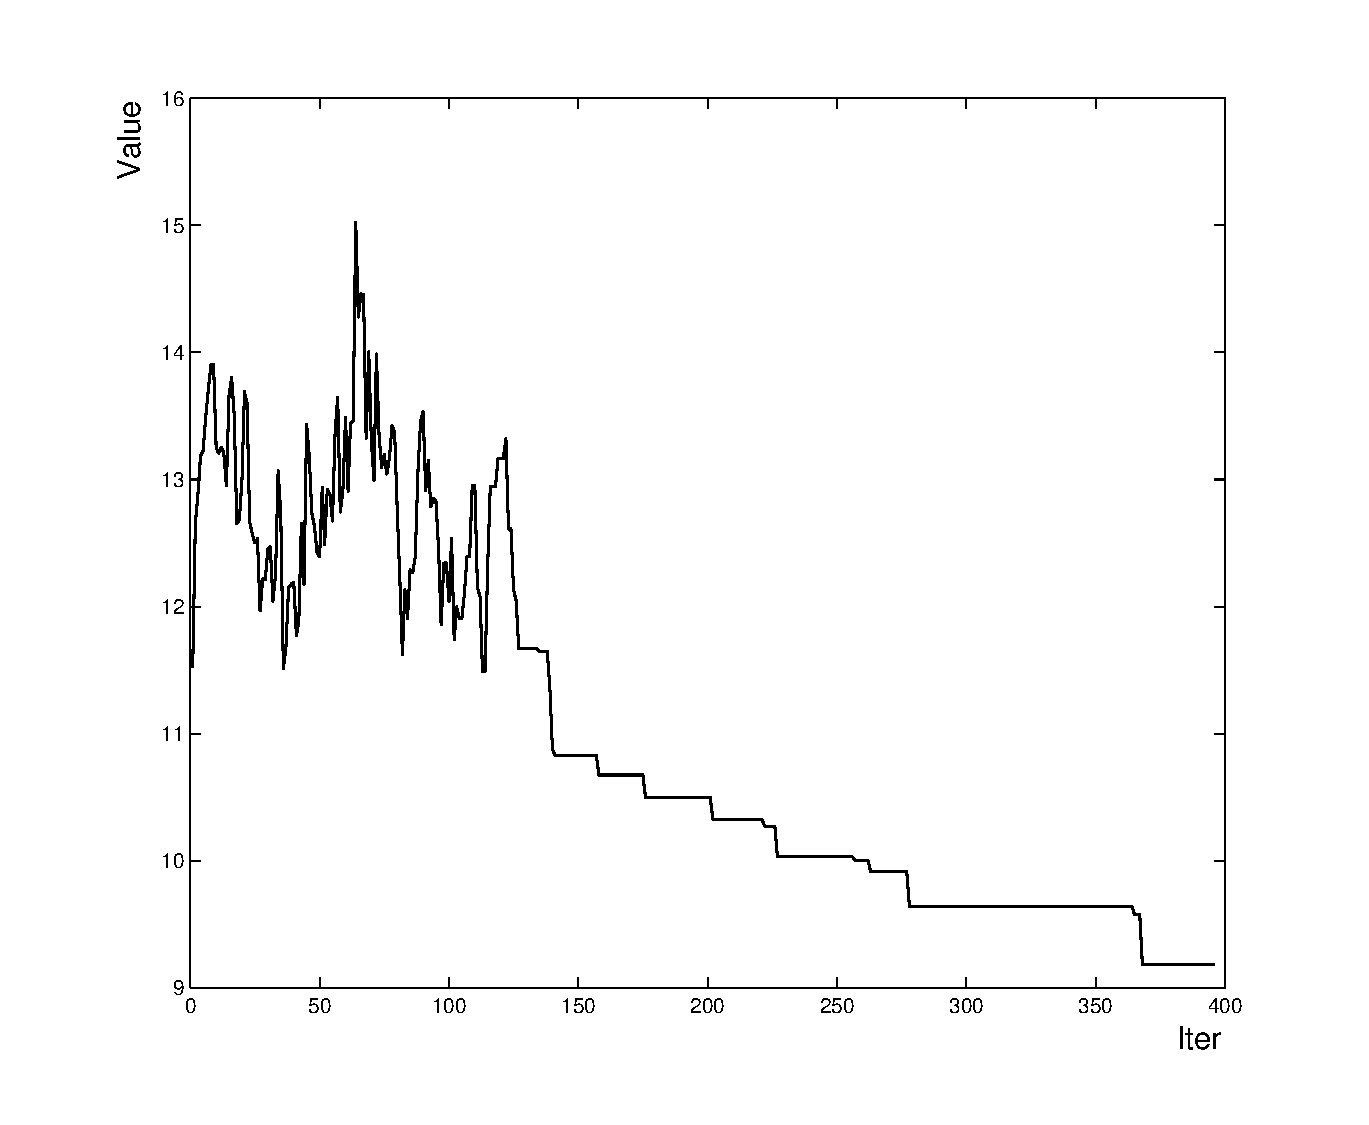
\includegraphics[width=0.8\textwidth]{figures/feasibility.eps}
\caption{算法收敛} \label{fig:feas}
\end{figure}
\section{稳定性}
我们已经看到算法可以成功收敛,但是如果每次收敛的结果差距过大则说明算法并不稳定,即不能保证每次都能得到一个较好的解。从表\ref{tab:stability}我们可以看到,当取$N_v = 100, N_p = 100$时,十组不同数据的测试最终收敛的结果非常相近,并且都是较好的解。说明算法具有一定的稳定性,对初值并不敏感。

\begin{table}[htbp]
  \centering
  \small
  \begin{threeparttable}
    \caption{\label{tab:stability}算法稳定性}
    \begin{tabular}{cccccc}
      \toprule
        & 评价 & PM使用率 & RAM均衡负载 & CPU均衡负载 & 平均冲突率 \\
      \midrule
      1 & 4.019 & 0.760 & 0.184 & 0.270 & 1.061 \\
      2 & 3.692 & 0.770 & 0.241 & 0.180 & 1.110 \\
      3 & 4.643 & 0.810 & 0.210 & 0.256 & 1.064 \\
      4 & 4.052 & 0.740 & 0.271 & 0.174 & 1.165 \\
      5 & 4.126 & 0.730 & 0.254 & 0.214 & 1.039 \\
      6 & 4.360 & 0.740 & 0.245 & 0.222 & 1.081 \\
      7 & 3.609 & 0.810 & 0.165 & 0.266 & 1.012 \\
      8 & 3.145 & 0.790 & 0.166 & 0.240 & 1.000 \\
      9 & 4.433 & 0.770 & 0.220 & 0.251 & 1.045 \\
     10 & 3.442 & 0.770 & 0.194 & 0.230 & 1.000 \\
      \bottomrule
    \end{tabular}
    \tiny
    \begin{tablenotes}
    \item [1]$N_v = 100,N_p = 100$

    \item [2] Using Simulated Annealing Algorithm \ref{algo:SA}
    \end{tablenotes}
  \end{threeparttable}
\end{table}

\section{实验结果}
我们选取了$100$到$1000$步长为$100$的十组数据规模,分别使用SA算法\ref{algo:SA}和FF算法对同一组数据进行计算,并取10次不同数据的平均值得到了表\ref{tab:result}:

\begin{table}[htbp]
  \centering
  \small
  \begin{threeparttable}
    \caption{\label{tab:result}测试数据}
    \begin{tabular}{clcccc}
      \toprule
数据规模       & 方法 & PM使用率 & RAM均衡负载 & CPU均衡负载 & 平均冲突率 \\
      \midrule
$ N_v = 100 $ & SA & 0.780 & 0.207 & 0.221 & 1.072 \\ 
              & FF & 0.920 & 0.247 & 0.297 & N/A \\
\hline 
$ N_v = 200 $ & SA & 0.770 & 0.230 & 0.220 & 1.061 \\
              & FF & 0.895 & 0.236 & 0.293 & N/A \\ 
\hline
$ N_v = 300 $ & SA & 0.773 & 0.245 & 0.212 & 1.087 \\ 
              & FF & 0.903 & 0.248 & 0.277 & N/A \\
\hline
$ N_v = 400 $ & SA & 0.785 & 0.239 & 0.249 & 1.082 \\
              & FF & 0.860 & 0.250 & 0.285 & N/A \\
\hline
$ N_v = 500 $ & SA & 0.792 & 0.236 & 0.234 & 1.090 \\ 
              & FF & 0.880 & 0.244 & 0.287 & N/A \\
\hline
$ N_v = 600 $ & SA & 0.797 & 0.236 & 0.235 & 1.095 \\
              & FF & 0.873 & 0.248 & 0.287 & N/A \\
\hline
$ N_v = 700 $ & SA & 0.801 & 0.249 & 0.259 & 1.101 \\
              & FF & 0.867 & 0.266 & 0.293 & N/A \\
\hline
$ N_v = 800 $ & SA & 0.814 & 0.239 & 0.253 & 1.097 \\ 
              & FF & 0.874 & 0.247 & 0.297 & N/A \\
\hline
$ N_v = 900 $ & SA & 0.793 & 0.246 & 0.251 & 1.101 \\ 
              & FF & 0.864 & 0.264 & 0.293 & N/A \\
\hline
$ N_v = 1000 $ & SA & 0.796 & 0.248 & 0.248 & 1.109 \\ 
               & FF & 0.871 & 0.271 & 0.291 & N/A \\

      \bottomrule
    \end{tabular}
  \end{threeparttable}
\end{table}

从实验获得的数据\ref{tab:result}中我们可以得到以下结论。

\subsection*{模拟退火算法是有效的}

First-Fit算法已经被证明是解决背包问题的一个高效的算法,从得到的数据中我们可以看到,我们设计的基于模拟退火算法得到的效果要好于FF得到的结果。

\subsection*{共享内存有效减少了PM的使用}
从表\ref{tab:result}中的数据我们可以看到,采用了内存可共享模型的SA算法可以有效减少PM的使用,比没有采用内存共享模型的FF平均要少$12\%$左右。同时,由于我们把平均冲突率作为因素之一引入了评价函数,算法可以将平均冲突率控制在1.1左右,即如果一台PM上的内存使用发生了冲突,冲突内存平均只占PM总内存的$10\%$,这个代价通常是可以被接受的。

\subsection*{SA算法能够获得负载均衡的解}
从表\ref{tab:result}中的数据我们可以看到,我们提出的算法可以有效控制系统的负载均衡,取得了比FF算法更好的结果。在实际问题中,更均衡的负载意味着更少的系统瓶颈,尤其是对网络通信任务比较繁重的系统来说,更均衡的负载可以明显提高服务的质量,减少延迟。

\subsection*{评价函数的重要性}
从得到的数据和上面的讨论可以看出,评价函数对本文所使用的算法的``优劣''有很大影响。但是,我们靠什么去评价一个解的优劣呢?显然不能以评价函数来评价---我们已经知道在评价函数下是好的了。因此,使用启发式算法来求解实际问题,应当是提出分析问题根据需求给出评价函数的模型,通过算法求解后代回问题观察是否在实际问题中理论上优的解真的有效,根据观察的结果不断的修正评价函数的模型才能获得理想的结果。






